\documentclass{article}
\usepackage[utf8]{inputenc}
\usepackage{caption}
\usepackage{subcaption}
\usepackage{graphicx}
\usepackage{hyperref}
\usepackage{pdflscape}
\usepackage[letterpaper, portrait, margin=1in]{geometry}
\renewcommand{\baselinestretch}{1.25}

\hypersetup{
    colorlinks=true,
    linkcolor=blue,
    urlcolor=blue,
    }
    
\usepackage[
    backend=biber,
    style=numeric,
    sorting=ynt
]{biblatex}

\addbibresource{Exported Items.bib}

\title{BF528 Individual Project}
\author{Taylor Falk, hedgehog group}
\date{May 8th 2021}

\begin{document}

\maketitle
\section{Introduction}
For recreating one of our projects, I chose to perform the programmer and analyst steps for Project 2, "Bioinformatics Reanalysis of: \textit{Transcriptional Profile of Mammalian Cardiac Regeneration with mRNA-Seq}" \cite{omearaTranscriptionalReversionCardiac2015}. I originally served as the biologist for this project, so I was interested in comparing the original outputs I worked on for the project to the work I could perform myself as programmer and analyst.

Repeating analyses is good scientific practice, not only for confirming experimental results, but also as a hands-on approach to analyzing the methods of a project. In performing the programmer and analyst steps once more, I can compare my results to those of my teammates and to the ultimate results achieved in the original paper, O'Meara et al. The original researchers sought to compare the transcriptional state of neonate and adult mouse heart tissue, as newborn and prenatal mammal hearts are known to have some regenerative processes after injury that developing and adult mammals do not possess. Both this and our original reanalysis replicated a comparison between the cardiac myocyte tissue from an adult (Ad) and zero-day post-natal mouse (P0).

\section{Methods}
A GitHub repository for this project can be found here: \url{https://github.com/taytayp/bf528_individual}

While not technically a part of this individual project, I did retrieve the SRA sample and convert to a FASTQ using SRA Toolkit as a part of the data curator's original task \cite{DownloadSoftwareSequence}. A new folder was created in our group directory, as the larger SRA and FASTQ files quickly fill up the allocated data in my home folder on Boston University's Shared Computing Cluster (SCC). In the interest of brevity, I did not perform the FASTQC steps, concluding that no significant issues were found with the original samples and no changes would be necessary for this reanalysis. I only analyzed sample P0 for this project, the zeroth-day post-natal neonate cardiac myocyte sample.


\begin{table}[!h]
\centering
\begin{tabular}{ll}
\hline
\multicolumn{2}{|c|}{Flagstat data}                                                    \\ \hline\hline
\multicolumn{1}{|l|}{Total reads}           & \multicolumn{1}{l|}{49,706,999}          \\ \hline
\multicolumn{1}{|l|}{Reads mapped}          & \multicolumn{1}{l|}{41,389,334 (83.3\%)} \\ \hline
\multicolumn{1}{|l|}{Unaligned reads}       & \multicolumn{1}{l|}{0}                   \\ \hline
                                            &                                          \\ \hline
\multicolumn{2}{|c|}{\texttt{bam\_stat.py} data}                                                    \\ \hline\hline
\multicolumn{1}{|l|}{Multimapped reads}     & \multicolumn{1}{l|}{8,317,665 (16.7\%)}  \\ \hline
\multicolumn{1}{|l|}{Reads mapped in pairs} & \multicolumn{1}{l|}{27,972,916 (56.3\%)} \\ \hline
\multicolumn{1}{|l|}{QC failed reads}       & \multicolumn{1}{l|}{0}                   \\ \hline
\end{tabular}
\caption{Read quality control figures generated by Samtools \texttt{flagstat} and RSeQC \texttt{bam\_stat.py}}
\label{tab:flagstat}
\end{table}

I next aligned the two FASTQ files to the reference mouse genome, \texttt{mm9} \cite{MGSCv37Mm9Genome}. I used TopHat version 2.1.1 to perform the alignment, utilizing 16 cores on the SCC \cite{trapnellTopHatDiscoveringSplice2009}. I then used RSeQC version 3.0.0 to perform quality control analysis on the accepted hits from TopHat's alignment, including gene coverage and statistics on the generated BAM file \cite{RSeQCRNAseqQuality}. Next, Cufflinks 2.2.1 was used to map the aligned reads to the \textit{Mus musculus} genes of regions, again with 16 processor cores \cite{trapnellTranscriptAssemblyQuantification2010}. Some quality analysis was done using the Samtools version 0.1.19 \texttt{flagstat} command \cite{danecekTwelveYearsSAMtools2021}. Using the quantified gene fragments per kilobase per million mapped fragments (FPKM), I loaded the Cufflinks output into R version 4.0.2 to plot their distribution (\textbf{Figure \ref{fig:fpkm}}) \cite{rlang}. We finally used \texttt{cuffdiff}, from the same Cufflinks version, to identify differentially expressed genes between P0 and Ad, the cardiac myocyte from an adult \textit{Mus musculus}.

Finally, I replicated the data analyst procedure of comparing and functionally annotating the differentially expressed genes found by \texttt{cuffdiff}. Using the same R version as above, I found the top ten differentially expressed genes by lowest q-value, and plotted the distribution of all and significant differentially expressed genes by $\log_2$ fold change. Then, taking the negatively and positively expressed significant genes and filtering them to remove lower $\log_2$ fold change values, I downloaded the gene names as down and up-regulated genes respectively. The 500 or so genes in each list were then separately loaded into DAVID  for functional annotation \cite{huangSystematicIntegrativeAnalysis2009}.

While again not part of the scope of this individual project, I did replace some of the original biologist role's inputs with my newly generated data, and once more plotted some of the heat maps in order to compare results visually. The details of generating these heat maps can be found in the original GitHub \url{https://github.com/BF528/project-2-hedgehog}.


\begin{figure}[h]
     \centering
     \begin{subfigure}[b]{0.5\textwidth}
         \centering
         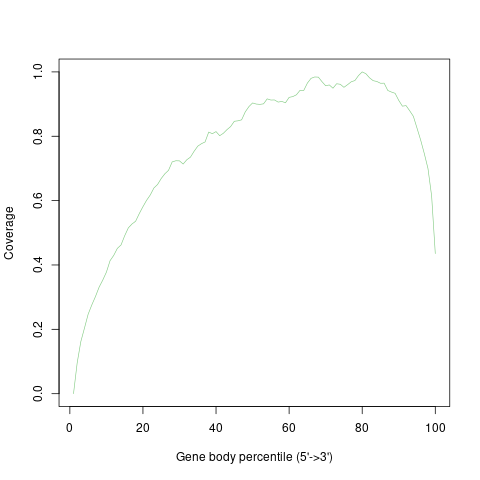
\includegraphics[width=0.9\textwidth]{plots/gene_coverage.png}
         \caption{The percentage of the gene body of \textit{Mus musculus} covered by the aligned reads.}
     \end{subfigure}%
     \hfill
     \begin{subfigure}[b]{0.5\textwidth}
         \centering
         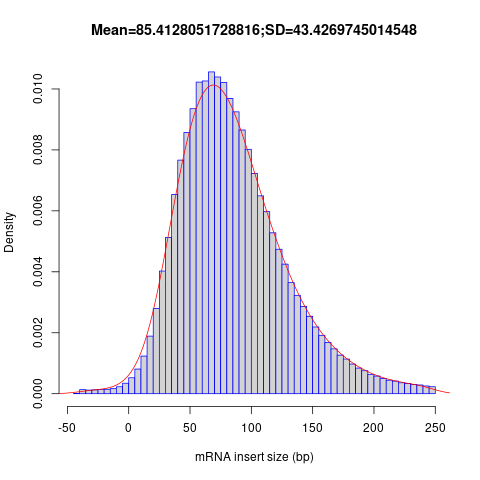
\includegraphics[width=0.9\textwidth]{plots/inner_distance.png}
         \caption{The distribution of RNA fragment insert sizes.}
     \end{subfigure}
     \hfill
        \caption{QC plots from RSeQC.}
        \label{fig:two graphs}
\end{figure}

\section{Results}

After aligning the accepted hits to the reference mouse genome, I used some quality control scripts to determine how well the mapping performed. No reads failed, and more than 80\% of the reads mapped to the referenced genome (\textbf{Table \ref{tab:flagstat}}). In order to further quantify the alignment, RSeQC plots were used to measure the coverage and fragment insert sizes, with no significant deviation from the first instance of this project (\textbf{Figure \ref{fig:two graphs}}).

Once the \texttt{Cufflinks} run for P0 was finished, I also plotted the distribution of non-zero FPKM counts. The distribution is very skewed, with a majority of the FPKM values falling under 100 fragments (\textbf{Figure \ref{fig:fpkm}}). 16,453 genes have non-zero FPKM values, of 37,469 total genes found (43.9\%). After using \texttt{cuffdiff}, I found the ten most differentially expressed genes between P0 and Ad, sorted by the q-value (\textbf{Table \ref{tab:topgenes}}).

\begin{table}[hb]
    \centering
    \begin{tabular}{|l|r|r|r|}
\hline
Gene & $\log_2$ fold change & p-value & q-value\\\hline\hline
Plekhb2 & 1.70481 & 0.00005 & 0.0010693\\\hline
Mrpl30 & 1.51794 & 0.00005 & 0.0010693\\\hline
Coq10b & 2.26901 & 0.00005 & 0.0010693\\\hline
Aox1 & 2.57682 & 0.00005 & 0.0010693\\\hline
Ndufb3 & 1.39851 & 0.00005 & 0.0010693\\\hline
Sp100 & 5.56218 & 0.00005 & 0.0010693\\\hline
Cxcr7 & 2.70247 & 0.00005 & 0.0010693\\\hline
Lrrfip1 & -2.27184 & 0.00005 & 0.0010693\\\hline
Ramp1 & -4.25594 & 0.00005 & 0.0010693\\\hline
Gpc1 & 1.85570 & 0.00005 & 0.0010693\\\hline
\end{tabular}
    \caption{The top ten differentially expressed genes.}
    \label{tab:topgenes}
\end{table}

After plotting the $\log_2$ fold change for all and then significant genes, I removed those genes that were not significant (p $< 0.01$) to filter the gene set (\textbf{Figure \ref{fig:log2fc}}). In order to select the most impactful genes, those genes which were not found to be significant were removed. 2,139 genes were found to be significant, with 1,084 of those being up-regulated and 1,055 being down-regulated.

I filtered the up and down-regulated genes to those with a $\log_2$ fold change above 2 and below -2, respectively, in order to filter to a more differentially expressed subset of genes. In the final set I used for functional annotation, there are 378 up-regulated genes and 640 down-regulated, significant genes (of the original 36,329 total). After functionally annotating these gene sets with DAVID, I found 194 clusters in the up-regulated gene set, and 270 clusters in the down-regulated set (\textbf{Tables \ref{tab:upreg}} and \textbf{\ref{tab:downreg}}).

\subsection{Comparison}
Since this individual project captures a brunt of the data preparation, and I originally performed the biologist role in the group version of this project, a good comparison of the group's and my methods would be to compare one of our final outputs together. The heat maps we originally generated compare the top 250 differentially expressed genes across all 8 samples. In recreating the heat map, there appears to be very little difference between the two outputs (\textbf{Figure \ref{fig:compare}}).

\begin{figure}[p]
    \centering
    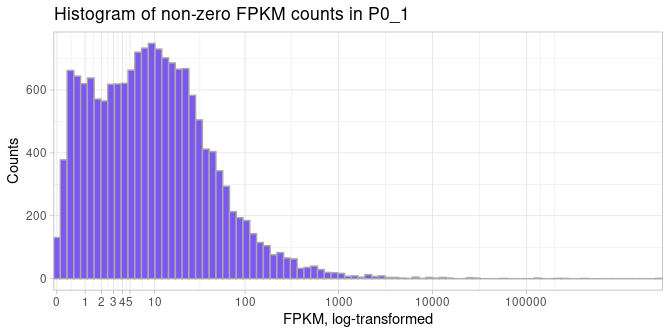
\includegraphics[width=\textwidth]{plots/Fig2-fpkm-histo.png}
    \caption{Distribution of FPKM counts higher than zero. x-axis log transformed to highlight number of genes with FPKM values under 100.}
    \label{fig:fpkm}
\end{figure}

\begin{figure}[p]
    \centering
    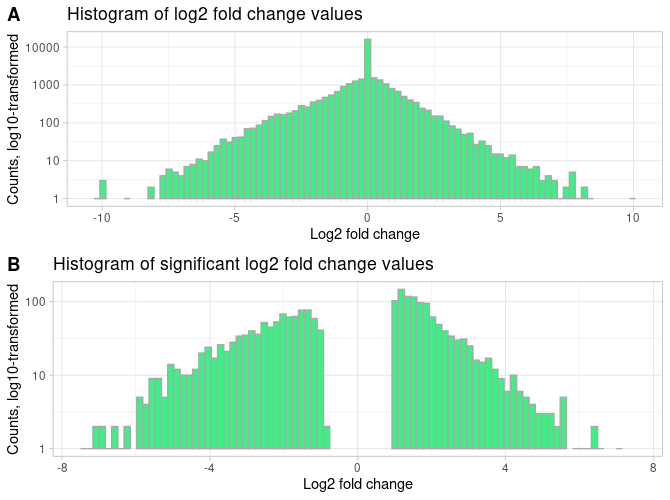
\includegraphics[width=\textwidth]{plots/log2fc.png}
    \caption{Distribution of $\log_2$ fold change values. Note the $\log_{10}$-transformed y-axes. A) The number of genes for each $\log_2$ fold change level. B) The same set of genes, with those not meeting the significance p-value (0.01) removed.}
    \label{fig:log2fc}
\end{figure}

\begin{landscape}
\begin{table}
\centering
\resizebox{\columnwidth}{!}{%
\begin{tabular}{|l|l|l|l|l|l|l|}
\hline
Category             & Term                                                               & PValue   & Fold Enrichment & Bonferroni & Benjamini & FDR      \\ \hline\hline
Annotation Cluster 1 & Enrichment Score: 7.246140277968392                                &          &                 &            &           &          \\ \hline
biological process   & GO:0052697$\sim$xenobiotic glucuronidation                         & 5.57E-14 & 5.87E+01        & 2.45E-10   & 2.45E-10  & 2.38E-10 \\ \hline
biological process   & GO:0009813$\sim$flavonoid biosynthetic process                     & 1.06E-09 & 2.52E+01        & 4.64E-06   & 5.16E-07  & 5.00E-07 \\ \hline
biological process   & GO:0052696$\sim$flavonoid glucuronidation                          & 1.06E-09 & 2.52E+01        & 4.64E-06   & 5.16E-07  & 5.00E-07 \\ \hline
biological process   & GO:0052695$\sim$cellular glucuronidation                           & 2.47E-09 & 2.30E+01        & 1.09E-05   & 1.09E-06  & 1.05E-06 \\ \hline
biological process   & GO:0006063$\sim$uronic acid metabolic process                      & 3.65E-09 & 2.20E+01        & 1.61E-05   & 1.34E-06  & 1.30E-06 \\ \hline
molecular function   & GO:0015020$\sim$glucuronosyltransferase activity                   & 8.77E-08 & 1.53E+01        & 8.06E-05   & 4.04E-05  & 3.93E-05 \\ \hline
molecular function   & GO:0008194$\sim$UDP-glycosyltransferase activity                   & 2.74E-03 & 3.77E+00        & 9.19E-01   & 1.14E-01  & 1.11E-01 \\ \hline
molecular function   & GO:0016757$\sim$transferase activity, transferring glycosyl groups & 8.67E-03 & 2.51E+00        & 1.00E+00   & 2.35E-01  & 2.29E-01 \\ \hline
molecular function   & GO:0016758$\sim$transferase activity, transferring hexosyl groups  & 2.01E-02 & 2.67E+00        & 1.00E+00   & 3.91E-01  & 3.80E-01 \\ \hline\hline
Annotation Cluster 2 & Enrichment Score: 6.474865240171514                                &          &                 &            &           &          \\ \hline
biological process   & GO:0006082$\sim$organic acid metabolic process                     & 5.98E-13 & 3.28E+00        & 2.63E-09   & 1.32E-09  & 1.28E-09 \\ \hline
biological process   & GO:0019752$\sim$carboxylic acid metabolic process                  & 1.34E-11 & 3.27E+00        & 5.91E-08   & 1.90E-08  & 1.84E-08 \\ \hline
biological process   & GO:0043436$\sim$oxoacid metabolic process                          & 1.73E-11 & 3.24E+00        & 7.60E-08   & 1.90E-08  & 1.84E-08 \\ \hline
biological process   & GO:0032787$\sim$monocarboxylic acid metabolic process              & 3.79E-10 & 3.61E+00        & 1.67E-06   & 2.38E-07  & 2.31E-07 \\ \hline
biological process   & GO:0006631$\sim$fatty acid metabolic process                       & 6.40E-04 & 2.69E+00        & 9.40E-01   & 3.35E-02  & 3.25E-02 \\ \hline
biological process   & GO:0044255$\sim$cellular lipid metabolic process                   & 3.80E-03 & 1.80E+00        & 1.00E+00   & 1.05E-01  & 1.02E-01 \\ \hline
biological process   & GO:0006629$\sim$lipid metabolic process                            & 9.10E-03 & 1.59E+00        & 1.00E+00   & 1.90E-01  & 1.84E-01 \\ \hline
biological process   & GO:0008610$\sim$lipid biosynthetic process                         & 1.37E-01 & 1.51E+00        & 1.00E+00   & 8.93E-01  & 8.66E-01 \\ \hline\hline
$\cdots$ & $\cdots$ & $\cdots$ & $\cdots$ & $\cdots$ & $\cdots$ & $\cdots$ \\ \hline\hline
Annotation Cluster 6 & Enrichment Score: 4.8607784926257125                               &          &                 &            &           &          \\ \hline
cellular component   & GO:0043230$\sim$extracellular organelle                            & 4.07E-07 & 1.66E+00        & 1.67E-04   & 1.67E-04  & 1.54E-04 \\ \hline
cellular component   & GO:1903561$\sim$extracellular vesicle                              & 1.43E-06 & 1.63E+00        & 5.83E-04   & 2.92E-04  & 2.70E-04 \\ \hline
cellular component   & GO:0070062$\sim$extracellular exosome                              & 2.19E-06 & 1.62E+00        & 8.95E-04   & 2.98E-04  & 2.76E-04 \\ \hline
cellular component   & GO:0031988$\sim$membrane-bounded vesicle                           & 6.96E-05 & 1.43E+00        & 2.81E-02   & 4.45E-03  & 4.11E-03 \\ \hline
cellular component   & GO:0044421$\sim$extracellular region part                          & 2.08E-04 & 1.36E+00        & 8.17E-02   & 1.00E-02  & 9.28E-03 \\ \hline
cellular component   & GO:0005576$\sim$extracellular region                               & 3.72E-04 & 1.31E+00        & 1.41E-01   & 1.38E-02  & 1.28E-02 \\ \hline
\end{tabular}%
}
\caption{Up-regulated genes functionally clustered into GO terms using DAVID. Some terms in clusters 1 and 2 were abbreviated, and clusters 3 through 5 were removed to include the cellular components in cluster 6.}
\label{tab:upreg}
\end{table}
\end{landscape}

\begin{landscape}
\begin{table}
\centering
\resizebox{\columnwidth}{!}{%
\begin{tabular}{|l|l|l|l|l|l|l|}
\hline
Category             & Term                                                      & PValue   & Fold Enrichment & Bonferroni & Benjamini & FDR      \\ \hline\hline
Annotation Cluster 1 & Enrichment Score: 10.393093321266553                      &          &                 &            &           &          \\ \hline
cellular component   & GO:0005694$\sim$chromosome                                & 5.90E-13 & 2.50E+00        & 3.33E-10   & 3.33E-10  & 3.13E-10 \\ \hline
cellular component   & GO:0000793$\sim$condensed chromosome                      & 1.93E-12 & 4.80E+00        & 1.09E-09   & 5.44E-10  & 5.13E-10 \\ \hline
cellular component   & GO:0044427$\sim$chromosomal part                          & 1.53E-11 & 2.50E+00        & 8.63E-09   & 2.88E-09  & 2.71E-09 \\ \hline
cellular component   & GO:0098687$\sim$chromosomal region                        & 3.56E-11 & 3.65E+00        & 2.01E-08   & 5.03E-09  & 4.73E-09 \\ \hline
cellular component   & GO:0000775$\sim$chromosome, centromeric region            & 5.85E-11 & 4.83E+00        & 3.30E-08   & 6.60E-09  & 6.22E-09 \\ \hline
cellular component   & GO:0000779$\sim$condensed chromosome, centromeric region  & 1.46E-10 & 6.16E+00        & 8.25E-08   & 1.38E-08  & 1.30E-08 \\ \hline
cellular component   & GO:0000777$\sim$condensed chromosome kinetochore          & 9.43E-10 & 6.29E+00        & 5.32E-07   & 6.65E-08  & 6.26E-08 \\ \hline
cellular component   & GO:0000776$\sim$kinetochore                               & 1.43E-09 & 5.44E+00        & 8.05E-07   & 8.94E-08  & 8.42E-08 \\ \hline\hline
Annotation Cluster 2 & Enrichment Score: 9.938373906529277                       &          &                 &            &           &          \\ \hline
biological process   & GO:0008283$\sim$cell proliferation                        & 6.29E-14 & 2.12E+00        & 3.32E-10   & 2.77E-11  & 2.58E-11 \\ \hline
biological process   & GO:0042127$\sim$regulation of cell proliferation          & 4.84E-11 & 2.06E+00        & 2.55E-07   & 1.34E-08  & 1.25E-08 \\ \hline
biological process   & GO:0008284$\sim$positive regulation of cell proliferation & 5.03E-07 & 2.11E+00        & 2.65E-03   & 4.82E-05  & 4.50E-05 \\ \hline\hline
Annotation Cluster 3 & Enrichment Score: 8.101617012505335                       &          &                 &            &           &          \\ \hline
biological process   & GO:0007049$\sim$cell cycle                                & 3.18E-30 & 3.13E+00        & 1.68E-26   & 1.68E-26  & 1.57E-26 \\ \hline
biological process   & GO:0000278$\sim$mitotic cell cycle                        & 7.61E-28 & 4.01E+00        & 4.01E-24   & 2.01E-24  & 1.87E-24 \\ \hline
biological process   & GO:1903047$\sim$mitotic cell cycle process                & 1.21E-27 & 4.23E+00        & 6.40E-24   & 2.13E-24  & 1.99E-24 \\ \hline
biological process   & GO:0051301$\sim$cell division                             & 7.06E-26 & 4.61E+00        & 3.73E-22   & 9.32E-23  & 8.70E-23 \\ \hline
biological process   & GO:0022402$\sim$cell cycle process                        & 1.26E-25 & 3.28E+00        & 6.64E-22   & 1.33E-22  & 1.24E-22 \\ \hline
biological process   & GO:0007067$\sim$mitotic nuclear division                  & 1.52E-21 & 4.85E+00        & 8.01E-18   & 1.33E-18  & 1.25E-18 \\ \hline\hline
Annotation Cluster 4 & Enrichment Score: 7.432059188879914                       &          &                 &            &           &          \\ \hline
biological process   & GO:0006259$\sim$DNA metabolic process                     & 3.36E-12 & 2.65E+00        & 1.77E-08   & 1.04E-09  & 9.73E-10 \\ \hline
biological process   & GO:0006974$\sim$cellular response to DNA damage stimulus  & 3.95E-08 & 2.51E+00        & 2.09E-04   & 5.96E-06  & 5.56E-06 \\ \hline
biological process   & GO:0033554$\sim$cellular response to stress               & 3.44E-06 & 1.71E+00        & 1.80E-02   & 2.04E-04  & 1.91E-04 \\ \hline
biological process   & GO:0006281$\sim$DNA repair                                & 4.09E-06 & 2.64E+00        & 2.14E-02   & 2.30E-04  & 2.14E-04 \\ \hline
\end{tabular}%
}
\caption{Down-regulated genes functionally clustered into GO terms using DAVID. Some clusters' terms were abbreviated or removed.}
\label{tab:downreg}
\end{table}
\end{landscape}

\begin{landscape}
\begin{figure}
     \centering
     \begin{subfigure}[b]{0.68\textwidth}
         \centering
         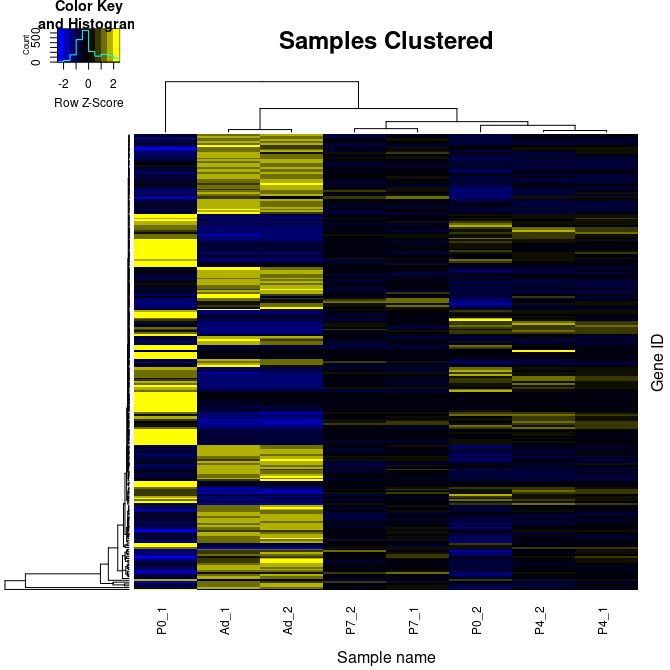
\includegraphics[width=\textwidth]{plots/clustered_v1.png}
         \caption{Version 1, generated before this project.}
     \end{subfigure}%
     \hfill
     \begin{subfigure}[b]{0.68\textwidth}
         \centering
         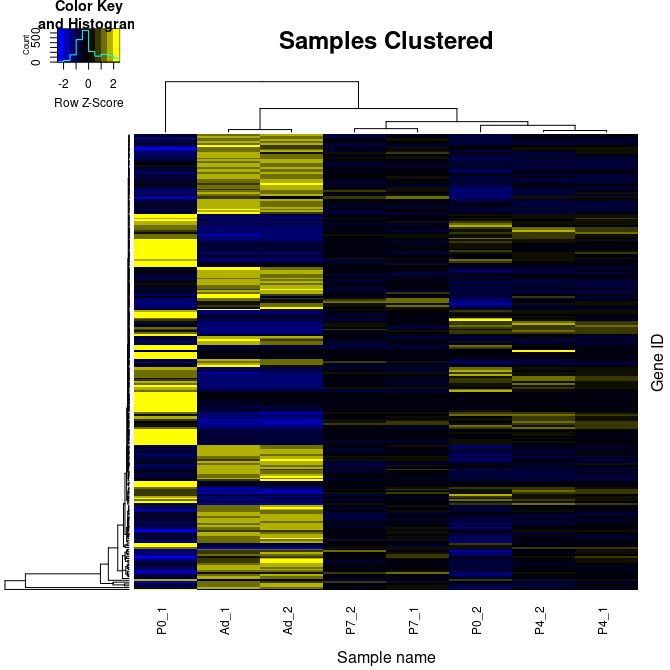
\includegraphics[width=\textwidth]{plots/clustered_v2.png}
         \caption{Version 2, from this project.}  
     \end{subfigure}
        \caption{Heat maps generated using biologist's code, from both reanalyses. 250 genes are included.}
        \label{fig:compare}
\end{figure}
\end{landscape}

\section{Discussion}
My goal for this reanalysis was to attempt to reproduce and compare our group's results in reanalyzing \textit{Transcriptional Profile of Mammalian Cardiac Regeneration with mRNA-Seq}. Not only was I able to recreate the exact same output figure, my alignment statistics were similar to the reported numbers from our original paper. I also sought to make some improvements, such as including some suggestions for figure and paper formatting, and applying some axis transformations to make plots more readable and detailed (such as \textbf{Figure \ref{fig:log2fc}A}). I also sought to improve the DAVID functional annotation of the data analyst section by reducing the number of genes included in the clustering, filtering on a higher $\log_2$ fold change value ($\pm$2 instead of 0). I was able to cluster up-regulated terms related to mitochondria and metabolism, and down-regulated terms related to the cell cycle. These were similar to our original functional annotation results, and those results of the source paper.

Ultimately, there is still an error in replicating the original O'Meara et al. paper since P0\_1 does not cluster near P0\_2 in \textbf{Figure \ref{fig:compare}}, but it is a good sign that the two plots are so similar. This likely hints at our group's original criticism of the heat map and earlier methodology being less reliable for an accurate recreation of these parts the original methods, and suggests that my own individual processing of the programmer and analyst steps mirrors my groups' original procedure.

\printbibliography

\end{document}
